% !TeX root = main.tex

\section{上同调理论}

\subsection{Hom 函子和单纯上同调}

我们考虑 Abel 群之间的群同态:

\begin{Definition}[Hom 函子]
	设 $ A, G $ 都是 Abel 群, 记 $ A $ 到 $ G $ 的群同态全体是 $ \Hom(A,G) $. $ G $ 上的加法结构可以诱导 $ \Hom(A,G) $ 上的加法结构如下:
	\[
		(f+g)(a):=f(a)+g(a).
	\]
	于是 $ (\Hom(A,G),+) $ 构成一个 Abel 群. 此时, 群同态 $ h : A\to B $ 可以如下诱导一个 $ \Hom(B,G) $ 到 $ \Hom(A,G) $ 的同态:
	\[
		\varphi h : A\stackrel{h}{\longrightarrow}B\stackrel{\varphi}{\longrightarrow}G\in\Hom(A,G),
	\]
	那么 $ \tilde{h}:=\Hom(h,G)=[\varphi\mapsto\varphi h] $ 是一个同态.
\end{Definition}

\begin{Proposition}
	$ \Hom : A\mapsto\Hom(A,G) $, $ h\mapsto \tilde{h} $ 给出了一个从 $ \category{Ab} $ 到 $ \category{Ab} $ 的反变函子.
\end{Proposition}
\begin{Proof}
	对 $ \id : A\to A $, $ \widetilde{\id}=\Hom(\id,G) $ 自然是 $ \Hom(A,G) $ 上的恒等映射. 而对 $ A\stackrel{h}{\to}B\stackrel{k}{\to}C $, 只需计算验证
	\[
		\widetilde{kh}(\varphi)=\varphi k h=\tilde{k}\varphi h=\tilde{h}\tilde{k}\varphi
	\]
	可知 $ \widetilde{kh}=\tilde{h}\tilde{k} $, 也即 $ \Hom $ 是一个反变函子.\qed
\end{Proof}

\begin{Proposition}\label{prop:Hom 保持正合且分裂}
	设 $ h $ 是一个 Abel 群同态, 那么
	\begin{enumerate}
		\item $ h $ 是同构 $ \Longrightarrow $ $ \tilde{h} $ 是同构;
		\item $ h=0\Longrightarrow\tilde{h}=0 $;
		\item $ h $ 是满同态 $ \Longrightarrow\tilde{h} $ 是单同态;
		\item 若序列
		\begin{center}
			\begin{tikzcd}
				0 \arrow[r] & A \arrow[r, "f"] & B \arrow[r, "g"] & C \arrow[r] & 0
			\end{tikzcd}
		\end{center}
		正合且分裂, 则序列
		\begin{center}
			\begin{tikzcd}
				0 & {\Hom(A,G)} \arrow[l] & {\Hom(B,G)} \arrow[l, "\tilde f"'] & {\Hom(C,G)} \arrow[l, "\tilde g"'] & 0 \arrow[l]
			\end{tikzcd}
		\end{center}
		也正合且分裂. 也即 $ f $ 是单同态推 $ \tilde{f} $ 是满同态需要添加序列分裂的条件.
	\end{enumerate}
\end{Proposition}
\begin{Proof}
	(1), (2) 的证明是容易的.

	(3) 任取 $ \varphi\in\Hom(B,G) $ 使得 $ \tilde{h}(\varphi)=\varphi h=0 $, 那么对任意 $ a\in A $ 成立
	\[
		\tilde{h}(\varphi(a))=\varphi h(a)=0,
	\]
	因 $ h $ 是满同态, 这即对任意 $ b\in B $ 有 $ \varphi(b)=0 $, 故 $ \varphi=0 $, 这说明 $ \tilde{h} $ 是单的.

	(4) 只需证明在 $ \Hom(B,G) $ 处正合, 也即 $ \im\tilde{g}=\ker\tilde{f} $.

	因第一个序列正合, 故 $ fg=0 $, 由 (2) 可知 $ \widetilde{gf}=\tilde{f}\tilde{g}=0 $. 于是 $ \im\tilde{g}\leqslant\ker\tilde{f} $. 再取 $ \varphi\in\ker\tilde{f}\leqslant\Hom(B,G) $, 由 $ \tilde{f}(\varphi)=\varphi f=0 $ 可知 $ \im f\leqslant\ker\varphi $, 那么
	\[
		\varphi' : B/\im f\to G
	\]
	是由 $ \varphi $ 诱导的群同态, 满足
	\begin{center}
		\begin{tikzcd}[row sep=huge]
			C & B \arrow[d] \arrow[l, "g"'] \arrow[r, "\varphi"]          & G \\
			  & B=\ker g=B/\im f \arrow[lu, "g'"] \arrow[ru, "\varphi'"'] &  
		\end{tikzcd}
	\end{center}
	因为 $ B\to C $ 是满同态, 于是 $ g' $ 是同构, 那么由交换图的可交换性得到
	\[
		\varphi=\varphi'(g')^{-1}g=\tilde{g}(\varphi'(g')^{-1})\in\im\tilde{g},
	\]
	于是 $ \ker\tilde{f}\leqslant\im\tilde{g} $.

	再考虑另一部分的证明. 因第一个序列分裂, 于是存在 $ \pi : B\to A $ 使得 $ \pi f=\id_A $, 那么 $ \widetilde{\pi f}=\widetilde{\id}_A $, 也即 $ \tilde{f}\tilde{\pi}=\widetilde{\id}_A $, 故 $ \tilde{f} $ 满, $ \tilde{\pi} $ 单, 并且第二个序列也是分裂的.\qed
\end{Proof}

在 (4) 中如果去掉序列分裂的条件, 那么结论往往不成立. 考虑 $ h : \Z\stackrel{\times 2}{\longrightarrow}\Z $, 这是一个单同态, 那么 $ \tilde{h} : \Hom(\Z,\Z)\stackrel{\tilde{2}}{\longrightarrow}\Hom(\Z,\Z) $, 对 $ \varphi : \Z\to\Z $ 是一个同态, 就有
\[
	\tilde{2}\varphi=\varphi(\times 2)=2\varphi,
\]
而 $ \Hom(\Z,\Z)\cong\Z $, 容易看出 $ \tilde{h} $ 并不是满同态.

\begin{Proposition}\label{prop:Hom 函子的直积性质}
	设 $ A,G,A_i,G_i $ 是 Abel 群, 则
	\begin{enumerate}
		\item $ \Hom(\bigoplus_{i\in\alpha}A_i,G)\cong\prod_{i\in\alpha}\Hom(A_i,G) $;
		\item $ \Hom(A,\prod_{i\in\alpha}G_i)\cong\prod_{i\in\alpha}\Hom(A,G_i) $.
	\end{enumerate}
\end{Proposition}
\begin{Proof}
	(1) 对 $ f : \bigoplus_{i\in\alpha}A_i\to G $, 取 $ f_i=f|_{A_i} $, 那么 $ \varPhi : f\mapsto\prod_{i\in\alpha}f_i $ 就是一个 $ \Hom(\bigoplus_{i\in\alpha}A_i,G)\to\prod_{i\in\alpha}\Hom(A_i,G) $ 的同态.

	反之, 对 $ f=\prod_{i\in\alpha}f_i $, $ f_i : A_i\to G $, 定义 $ \varPsi(f) : \bigoplus_{i\in\alpha}A_i\to G $ 满足 $ \varPsi(f)(a)=\sum_{i\in\alpha}f_i(a_i) $ 即可. 这里限制到代数直和是因为有限和的限制让我们无需考虑级数.

	(2) 类似.\qed
\end{Proof}

\begin{Proposition}
	设 $ G $ 是 Abel 群, 则
	\[
		\Hom(\Z,G)\cong G,\qquad\Hom(\Z/m\Z,G)\cong\ker[G\stackrel{m}{\longrightarrow}G].
	\]
\end{Proposition}
\begin{Proof}
	第一个断言取
	\[
		\lambda : \Hom(\Z,G)\to G,\qquad \varphi\mapsto\varphi(1)
	\]
	就是一个同构. 而对第二个断言, 由于序列
	\begin{center}
		\begin{tikzcd}
			0 \arrow[r] & \Z \arrow[r, "m"] & \Z \arrow[r] & \Z/m\Z \arrow[r] & 0
		\end{tikzcd}
	\end{center}
	正合, 那么
	\begin{center}
		\begin{tikzcd}
			0 & {\Hom(\Z,G)} \arrow[l] & {\Hom(\Z,G)} \arrow[l, "\tilde m"'] & {\Hom(\Z/m\Z,G)} \arrow[l, "\tilde\varphi"'] & 0 \arrow[l]
		\end{tikzcd}
	\end{center}
	也是正合的. 这里 $ \tilde{\varphi} $ 是单同态导出了 $ \Hom(\Z/m\Z,G)\cong\im\varphi $, 而序列正合导出了 $ \im\tilde{\varphi}\cong\ker\tilde{m} $.\qed
\end{Proof}

在单纯同调理论中, 我们通过单纯链复形 $ \CC $ 导出了单纯同调群 $ H_p(\CC) $. 那么 $ \Hom $ 函子作用之后的 $ \Hom(\CC;G) $, 我们希望它也对偶地导出同调群.

对单纯复形 $ K $, 考虑如下导出的链群:
\begin{center}
	\begin{tikzcd}
		& {\CC(K)=\set{(C_p(K),\partial)}} \arrow[dd, "{\Hom(\cdot,G)}"] \arrow[r] & H_p(\CC(K)) \\
K \arrow[ru] \arrow[rd] &                                                                          &             \\
		& {\Hom(\CC(K);G)=\set{(C^p(K;G),\delta)}} \arrow[r]                       & H^p(\CC(K))
	\end{tikzcd}
\end{center}~\\
称 $ \Hom(C_p(K),G):=C^p(K;G) $ 是 $ p $ 维\emph{上链群}, 这里的 $ \delta=\Hom(\partial,G) $.

\begin{Proposition}
	$ \Hom(\CC(K),G) $ 仍是一个链复形, 它以 $ \delta=\Hom(\partial,G) $ 为边缘算子.
\end{Proposition}
\begin{Proof}
	考虑
	\[
		\delta : C^p(K;G)\to C^{p+1}(K;G),\qquad c^p\mapsto\delta c^p=\tilde{\partial}c^p=c^p\delta,
	\]
	这里 $ \delta c^p : C_{p+1}(K)\to C_p(K) $. 并且
	\[
		\delta c^p(c_{p+1})=c^p(\partial c_{p+1})
	\]
	可以看作是 $ c^p $ 作用于 $ c_{p+1} $ 上的值, 于是我们把它写成类似于内积的形式: $ \lrangle{\delta c^p,c_{p+1}}=\lrangle{c^p,\partial c_{p+1}} $.
	
	而 $ \delta^2=0 $ 由 $ \partial^2=0 $ 立刻得到.\qed
\end{Proof}

于是可以在 $ \Hom(\CC(K),G) $ 上定义上同调. 记
\[
	\ker\delta_p:=Z^p(K;G),\qquad \im\delta_{p+1}:=B^p(K;G),
\]
称
\[
	H^p(K;G)=Z^p(K;G)/B^p(K;G)
\]
是 $ K $ 的 $ p $ 维\emph{上同调群}. (\textit{这里称作上同调完全是因为此时习惯把指标写在右上角, cohomology 的 co-- 前缀表示代数对偶}).

对任何 Abel 群 $ G $, 它有自由部分(\textit{以 $ \Z $ 为直和项})和挠部分(\textit{以 $ \Z/m\Z $ 为直和项}), 而之前已经讨论过
\[
	\Hom(\Z,G)\cong G,\qquad \Hom(\Z/m\Z,G)\cong\ker[G\stackrel{m}{\to}G].
\]

我们需要注意, 由
\[
	C^p(K;G)\cong\Hom(C_p(K),G)\cong\Hom\Big( \bigoplus_{\sigma\in S_p^+(K)}\Z\lrangle{\sigma},G \Big)\cong\prod_{\sigma\in\S_p^+(K)}\Hom(\Z\lrangle{\sigma},G)
\]
未必是一个自由 Abel 群.

要计算 $ H^p(K;G) $, 就归结到计算 $ \delta c $ 的问题, 所以下面处理上链如何表达. 在单纯同调理论中, 有 $ p $ 维基本链 $ \sigma_\alpha\in S_p^+(K) $, 类似地, 我们希望也有 $ p $ 维基本上链.

先考虑 $ G=\Z $ 的情形, 此时对 $ \sigma_\beta\in S_p^+(K) $, 定义
\[
	\lrangle{\sigma_\alpha^*,\sigma_\beta}:=\begin{cases}
		1 & ,\beta=\alpha \\ 0 & ,\beta\ne\alpha
	\end{cases}
\]
那么对任何 $ c^p\in C^p(K;\Z)=:C^p(K) $, 就有 $ c^p=\sum_{\alpha}n_\alpha\sigma_\alpha^* $. (\textit{这里的和未必是有限和}). 对一般的 Abel 群 $ G $, 我们考虑 $ g_\alpha\sigma_\alpha^* $, 这里 $ g_\alpha\in G $. 之前把它写成内积的形式, 我们同样希望这里的 ``内积'' 保持双线性, 于是可以定义
\[
	\lrangle{g_\alpha\sigma_\alpha^*,\sigma_\beta}:=\begin{cases}
		g_\alpha & ,\beta=\alpha \\ 0 & ,\beta\ne\alpha
	\end{cases}
\]
那么对任何 $ c^p\in C^p(K;\Z)=:C^p(K) $, 就有 $ c^p=\sum_{\alpha}g_\alpha\sigma_\alpha^* $. (\textit{同样地, 这里的和未必是有限和}).

\begin{Proposition}
	对 $ c^p=\sum_{\alpha}g_\alpha\sigma_\alpha^* $, 有 $ \delta c^p=\sum_{\alpha}g_\alpha\delta\sigma_\alpha^* $.
\end{Proposition}
\begin{Proof}
	对 $ \tau\in S_{p+1}^+(K) $, 有 $ \delta\tau=\sum_{i=0}^{p+1}\varepsilon_i\sigma_i $, 其中 $ \varepsilon_i=\pm 1 $, 取决于 $ \sigma_i $ 的定向. (\textit{这因低维单形的定向未必总是与高维单形定向相同}). 此时
	\[
		\lrangle{\delta c^p,\tau}=\lrangle{\sum_{\alpha}g_\alpha\sigma_\alpha^*,\sum_{i=0}^{p+1}\varepsilon_i\sigma_i}=\sum_{\alpha}\sum_{i=0}^{p+1}g_\alpha\varepsilon_i\lrangle{\sigma_\alpha^*,\sigma_i}=\sum_{i=0}^{p+1}\varepsilon_i g_i.
	\]
	而
	\[
		\lrangle{\sum_{\alpha}g_\alpha\delta\sigma_\alpha^*,\tau}=\sum_{i=0}^{p+1}\varepsilon_i g_i.
	\]
	这说明在每一个单形 $ \tau $ 上 $ c^p=\sum_{\alpha}g_\alpha\sigma_\alpha^* $, 于是命题得证.\qed
\end{Proof}

由这一条件, 在几何上, $ \delta\sigma_\alpha^* $ 的计算可以简单地遵从下面的规则. 记 $ \tau_i $ 是所有以 $ \sigma_\alpha $ 为面的单形, 则
\[
	\delta\sigma_\alpha^*=\sum_{i}\varepsilon_i\tau_i^*,
\]
这里 $ \varepsilon_i $ 是 $ \sigma_\alpha $ 在 $ \partial\tau_i $ 中的系数.
\newpage
\begin{Example}\label{ex: 一个计算例子}
	考虑下面的 2 维单纯复形
	\begin{figure}[h]
		\centering
		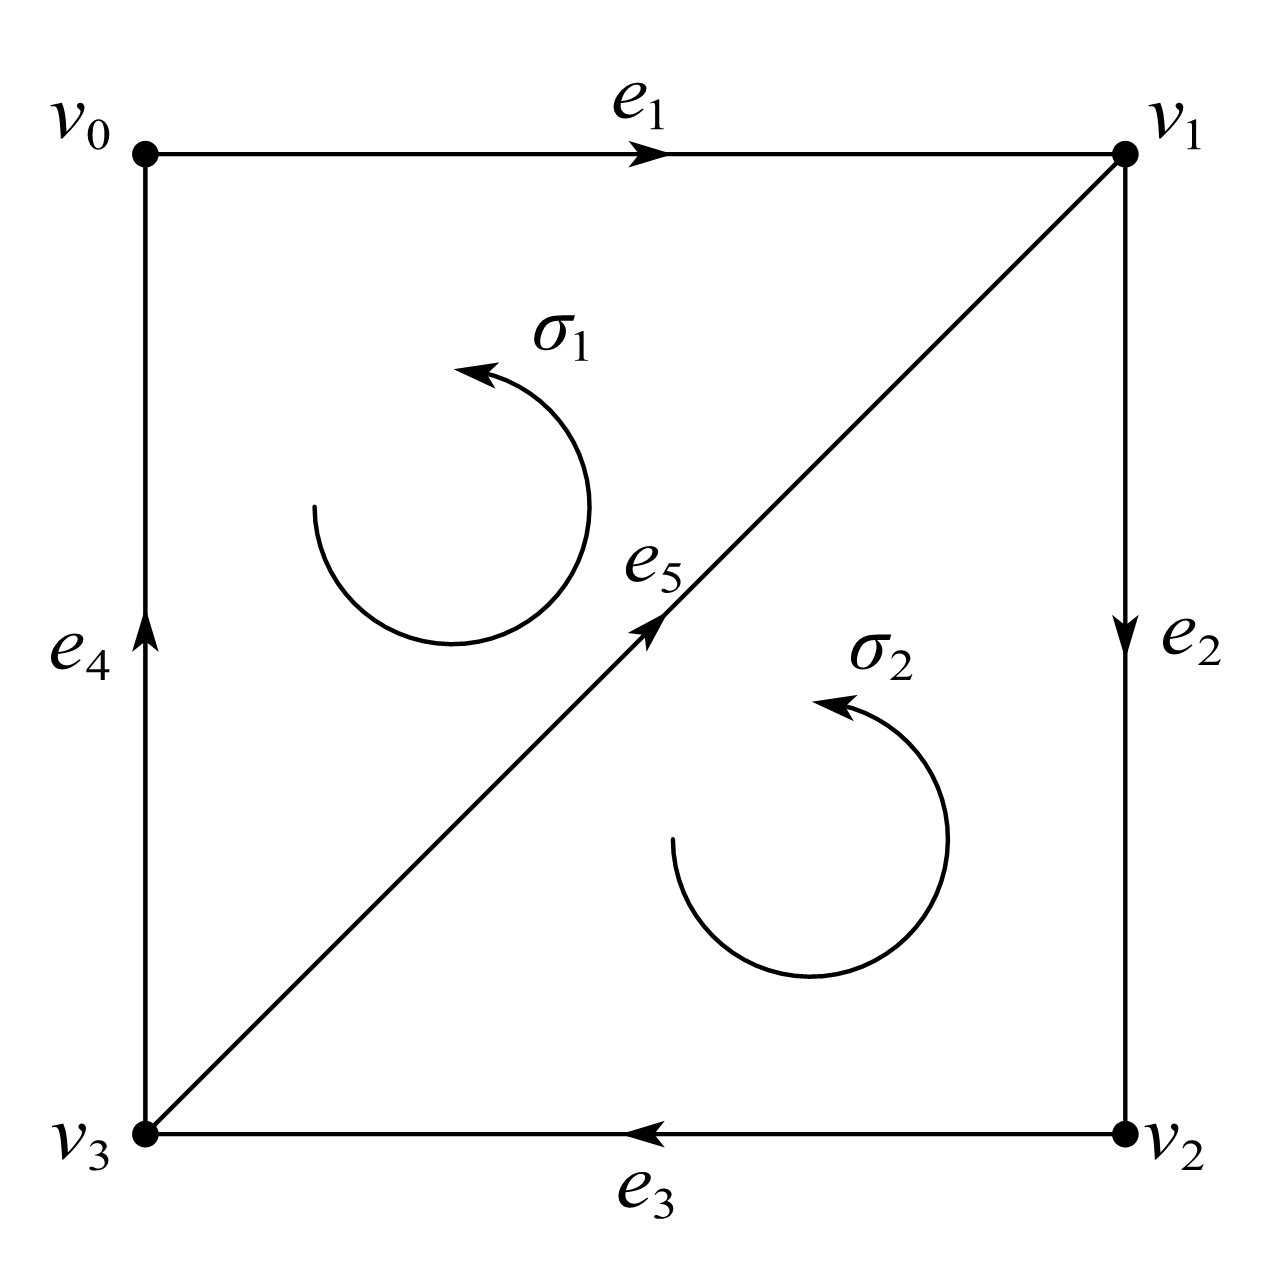
\includegraphics[width=0.25\linewidth]{figures/Sec15-1.png}
	\end{figure}

	只需分别计算不同维数的基本上链的边缘即可. 对 2--基本上链
	\[
		\delta\sigma_1^*=\delta\sigma_2^*=0,
	\]
	对 1--基本上链, 有
	\[
		\delta e_1^*=\delta e_4^*=-\sigma_1^*,\quad \delta e_2^*=\delta e_3^*=-\sigma_2^*,\quad \delta e_5^*=\sigma_1^*-\sigma_2^*.
	\]
	对 0--基本上链, 有
	\[
		\delta v_0^*=e_4^*-e_1^*,\quad \delta v_1^*=e_1^*-e_2^*+e_5^*,\quad \delta v_2^*=e_2^*-e_3^*,\quad \delta v_3^*=e_3^*-e_4^*-e_5^*.
	\]

	考虑 $ K $ 关于系数 $ \Z $ 的上同调群: 列出 $ K $ 的上链复形有
	\begin{center}
		\begin{tikzcd}
			0 & \Z\oplus\Z \arrow[l, "\delta_2"'] & \Z^{\oplus 4} \arrow[l, "\delta_1"'] & \Z^{\oplus 4} \arrow[l, "\delta_0"'] & 0 \arrow[l]
		\end{tikzcd}
	\end{center}
	那么 $ \im\delta_0=0 $ 导出 $ H^0(K)\cong\ker\delta_0=Z^0(K) $, 对任意 $ c^0=\sum_{i=0}^3n_iv_i^*\in C^0(K) $, 由
	\[
		\begin{aligned}
			\delta c^0=0&\Longleftrightarrow \sum_{i=0}^3n_i\delta v_i^*=0\\
			&\Longleftrightarrow (n_0-n_3)e_4^*+(n_1-n_0)e_1^*+(n_2-n_1)e_2^*+(n_3-n_2)e_3^*=0\\
			&\Longleftrightarrow n_0=n_1=n_2=n_3=n.
		\end{aligned}
	\]
	这就说明 $ Z^0(K)=\Z\lrangle{\sum_{i=0}^3v_i^*}\cong\Z $, 于是 $ H^0(K)\cong\Z $.

	再考虑 $ p=1 $ 的情形, $ Z^1(K)=\ker\delta_1 $, 对 $ c^1=\sum_{i=1}^5n_ie_i^*\in C^1(K) $, 类似地有
	\[
		\delta c^1=0\Longleftrightarrow\begin{cases}
			n_1=n_5-n_4\\ n_2=-n_3-n_5
		\end{cases}.
	\]
	于是对 $ c^1\in Z^1(K) $, 有
	\[
		\begin{aligned}
			c^1&=(n_5-n_4)e_1^*+(-n_3-n_5)e_2^*+n_3e_3^*+n_4e_4^*+n_5e_5^*\\
			&=n_3(e_3^*-e_2^*)+n_4(e_4^*-e_1^*)+n_5(e_1^*-e_2^*+e_5^*)\\
			&=-n_3\delta v_2^*+n_4\delta v_0^*+n_5\delta v_1^*,
		\end{aligned}
	\]
	这即 $ Z^1(K)=B^1(K) $, 于是 $ H^1(K)=Z^1(K)/B^1(K)=0 $.

	当 $ p=2 $ 时, 因 $ \ker\delta_2=C^2(K) $, 故 $ H^2(K)=C^2(K)/\im\delta_1=C^2(K)/B^2(K) $, 而
	\[
		\sigma_1^*=-\delta e_1^*,\qquad \sigma_2^*=\delta e_2^*
	\]
	说明 $ C^2(K)=B^2(K) $, 从而 $ H^2(K)=0 $. 其他阶上同调群自然为零.
\end{Example}
 
这样的计算无疑是低效而繁复的.

\begin{Proposition}
	设 $ K $ 是单纯复形, 有
	\[
		H^0(K;G)=\set{c^0\in C^0(K) : \forall v,w\text{\,位于\,}\abs{K}\text{\,的同一连通分支\,}, \lrangle{c^0,v}=\lrangle{c^0,w}}.
	\]
	特别地, 若 $ \abs{K} $ 连通, 就有 $ H^0(K;G)\cong G $.
\end{Proposition}
\begin{Proof}
	设 $ c^0 $ 满足条件, 要证 $ \delta c^0=0 $ 当且仅当对任意 $ \sigma=[v,w]\in S_1^+(K) $ 都有 $ \lrangle{\delta c^0,\sigma}=0 $.

	因
	\[
		\lrangle{\delta c^0,\sigma}=\lrangle{c^0,\partial\sigma}=\lrangle{c^0,w}-\lrangle{c^0,v}=0,
	\]
	于是 $ c^0\in\ker\delta_0=H^0(K;G) $.

	反之, 若 $ c^0\in\ker\delta_0 $, 即 $ \delta c^0=0 $, 则当 $ v,w $ 位于 $ \abs{K} $ 的同一连通分支时, 存在 $ c_1\in C_1(K) $ 使得 $ \partial c_1=w-v $, 那么
	\[
		0=\lrangle{\delta c^0,c_1}=\lrangle{c^0,\partial c_1}=\lrangle{c^0,w}-\lrangle{c^0,v},
	\]
	这即 $ \lrangle{c^0,w}=\lrangle{c^0,v} $.

	当 $ \abs{K} $ 连通时, 对任何 $ v,w\in K^{(0)} $, 应有 $ v,w $ 位于同一同调类中. 于是对任何 $ c^0=\sum_{v\in K^{(0)}}g_vv^*\in\ker\delta_0 $,
	\[
		g_v=\lrangle{c^0,v}=\lrangle{c^0,w}=g_w,
	\]
	这即 $ c^0=g\sum_{v\in K^{(0)}}v^* $, 从而 $ H^0(K;G)\cong G $.\qed
\end{Proof}

\begin{Definition}[约化上同调]
	对上链复形做增广, 得到
	\begin{center}
		\begin{tikzcd}
			{} & C^1(K;G) \arrow[l] & C^0(K;G) \arrow[l, "\delta_0"'] & {\Hom(\Z,G)\cong G} \arrow[l, "\tilde\varepsilon"']
		\end{tikzcd}
	\end{center}
	它导出的上同调群称作\emph{约化上同调群}, 并且容易得到 $ \tilde{H}^p(K;G)\cong H^p(K;G) $.
\end{Definition}

\begin{Proposition}
	$ \im\tilde{\varepsilon}\leqslant\ker\delta_0 $, 进一步 $ H^0(K;G)\cong\tilde{H}^0(K;G)\oplus G $.
\end{Proposition}
\begin{Proof}
	任取 $ \alpha\in\im\tilde{\varepsilon} $, 即存在 $ \varphi\in\Hom(\Z,G) $ 使得 $ \tilde{\varepsilon}(\varphi)=\alpha $, 那么
	\[
		\delta_0\alpha=\delta_0\tilde{\varepsilon}(\varphi)=\widetilde{\varepsilon\partial_1}(\varphi)=0,
	\]
	即 $ \alpha\in\ker\delta_0 $, 从而 $ \im\tilde{\varepsilon}\leqslant\ker\delta_0 $. 那么
	\[
		\ker\delta_0=\frac{\ker\delta_0}{\im\tilde{\varepsilon}}\oplus\im\tilde{\varepsilon}.
	\]

	那么这就是
	\[
		H^0(K;G)=\ker\delta_0=\frac{\ker\delta_0}{\im\tilde{\varepsilon}}\oplus\im\tilde{\varepsilon}=\tilde{H}^0(K;G)\oplus\Hom(\Z;G)\cong\tilde{H}^0(K;G)\oplus G.
	\]
	特别地, 当 $ \abs{K} $ 连通时 $ \tilde{H}^0(K;G)=0 $.\qed
\end{Proof}

对复形对 $ (K,K_0) $, 有
\[
	(K,K_0)\longrightarrow \CC(K,K_0)\longrightarrow \Hom(\CC(K,K_0),G),
\]
后者是一个链复形, 于是可以定义\emph{相对上同调群}
\[
	H^p(K,K_0;G):=Z^p(K,K_0;G)/B^p(K,K_0;G).
\]

注意到 $ C^p(K,K_0;G) $ 可以看作是 $ C^p(K;G) $ 的子群, 这因
\[
	\begin{aligned}
		C^p(K,K_0;G)E&=\set{f : C_p(K,K_0)\to G}\\
		&\cong\set{f : C_p(K)\to G : f|_{C_p(K_0)}=0}\leqslant C^p(K;G).
	\end{aligned}
\]
并且 $ C^p(K_0;G) $ 可以看作 $ C^p(K;G) $ 的商群, 考虑
\[
	\tilde{\imath} : C^p(K;G)\twoheadrightarrow C^p(K_0;G),\qquad \varphi\mapsto\tilde{\imath}(\varphi)=\varphi|_{C_p(K_0)}=\varphi i : C_p(K_0)\to G.
\]
由同态基本定理可知
\[
	C^p(K;G)/\ker\tilde{\imath}\cong C^p(K_0;G).
\]

在同调理论中有正合且分裂的序列
\begin{center}
	\begin{tikzcd}
		0 \arrow[r] & \CC(K_0) \arrow[r, "i"] & \CC(K) \arrow[r, "j"] & {\CC(K,K_0)} \arrow[r] & 0
	\end{tikzcd}
\end{center}
于是由~\ref{prop:Hom 保持正合且分裂}~可知序列
\begin{center}
	\begin{tikzcd}
		0 & {\Hom(\CC(K_0),G)} \arrow[l] & {\Hom(\CC(K),G)} \arrow[l, "\tilde{\imath}"] & {\Hom(\CC(K,K_0),G)} \arrow[l, "\tilde{\jmath}"] & 0 \arrow[l]
	\end{tikzcd}
\end{center}
仍然正合且分裂. 于是 zig--zag 引理导出长正合序列
\begin{center}
	\begin{tikzcd}
		{} & H^p(K_0;G) \arrow[l] & H^p(K;G) \arrow[l, "\tilde{\imath}^*"'] & {H^p(K,K_0;G)} \arrow[l, "\tilde{\jmath}^*"'] & H^{p-1}(K_0;G) \arrow[l, "\delta^*"'] & {} \arrow[l]
	\end{tikzcd}
\end{center}

\begin{Example}
	考虑~\ref{ex: 一个计算例子}~中相同的复形 $ K $, $ K_0 $ 是由 $ \set{v_i}_{i=1}^4 $ 和 $ \set{e_i}_{i=1}^4 $ 构成的子复形.

	注意到 $ K_0 $ 是 1 维子复形, 于是 $ H^2(K_0)=0 $. 由~\ref{ex: 一个计算例子}~我们已经得到 $ H^1(K)=H^2(K)=0 $, 于是长正合列
	\begin{center}
		\begin{tikzcd}
			{} & H^2(K) \arrow[l] & {H^2(K,K_0)} \arrow[l] & H^1(K_0) \arrow[l] & H^1(K) \arrow[l] & {} \arrow[l]
		\end{tikzcd}
	\end{center}
	导出 $ H^2(K,K_0)\cong H^1(K_0) $, 而 $ H^1(K_0) $ 是容易计算的.

	由 $ \dim K_0=1 $ 可知 $ Z^1(K_0)=C^1(K_0) $. 此时 $ e_1^*\sim e_2^*\sim e_3^*\sim e_4^* $, 于是 $ C^1(K_0)\cong\Z\lrangle{e_1^*} $. 而对任意 $ c^0\in C^0(K_0) $ 和 $ z=\sum_{i=1}^4e_i\in Z_1(K) $, 由
	\[
		\lrangle{\delta c^0,z}=\lrangle{c^0,\partial z}=0
	\]
	和
	\[
		\lrangle{ne_1^*,z}=n\lrangle{e_1^*,e_1}=n
	\]
	可知 $ B^1(K_0)=0 $. 从而 $ H^1(K_0)\cong\Z $, 因此 $ H^2(K,K_0)\cong\Z $.
\end{Example}

对一般链复形 $ \CC=\set{(C_p,\partial)} $, 这里 $ C_p $ 是 Abel 群, 它经过 Hom 函子之后得到的
\[
	\Hom(\CC,G)=\set{(\Hom(C_p,G),\delta)}=\set{(C^p(\CC;G),\delta)}
\]
仍然是一个链复形, 于是同样地可以定义上同调群 $ H^p(\CC;G):=\ker\delta_p/\im\delta_{p-1} $.

若 $ \CC $ 可以阶段, 适当地调整下标, 在被截断的地方放上一个 $ \Z $ 之后被 Hom 函子作用, 可以得到\emph{增广上链复形}, 于是也可以诱导约化同调群.

考虑链映射 $ f : \CC\to\CC' $ 满足 $ \partial'f=f\partial $, 那么经过 Hom 函子作用之后得到的
\[
	\tilde{f} : \Hom(\CC';G)\to\Hom(\CC;G)
\]
满足
\[
	\partial'f=f\partial\Longrightarrow\widetilde{\partial'f}=\widetilde{f\partial}\Longrightarrow\tilde{f}\delta'=\delta\tilde{f},
\]
它诱导 $ f^* : H^p(\CC';G)\to H^p(\CC;G) $.

同样地, 将链同伦的交换图表作 $ \Hom $ 函子之后, 我们自然地得到\emph{上链同伦}:
\begin{center}
	\begin{tikzcd}
		& C'^{p+1} \arrow[ld, "\tilde{D}"']       \\
		C^p   & C'^{p} \arrow[l, "\tilde{f}"', shift right] \arrow[l, "\tilde g", shift left] \arrow[u, "\delta'"'] \arrow[ld, "\tilde{D}"] \\
		C^{p-1} \arrow[u, "\delta"] &   
	\end{tikzcd}
\end{center}
它自然也满足 $ \tilde{D}\delta'-\delta\tilde{D}=\tilde g-\tilde f $. 并且同样满足同伦公理, 即 $ \tilde\varphi\simeq\tilde\psi\Longrightarrow\varphi^*=\psi^* $.

但对一般的链复形, 正合列
\begin{center}
	\begin{tikzcd}
		0 \arrow[r] & \CC \arrow[r] & \CD \arrow[r] & \CE \arrow[r] & 0
	\end{tikzcd}
\end{center}
未必是分裂的, 因为 $ \CC,\ \CD,\ \CE $ 未必是自由的. 因此无法推出序列
\begin{center}
	\begin{tikzcd}
		0 & {\Hom(\CC,G)} \arrow[l] & {\Hom(\CD,G)} \arrow[l] & {\Hom(\CE,G)} \arrow[l] & 0 \arrow[l]
	\end{tikzcd}
\end{center}
的正合性.

所以我们取一个简单的例子, 考虑空间对 $ (X,A) $ 的奇异链复形
\begin{center}
	\begin{tikzcd}
		0\arrow[r] & \CS(A)\arrow[r]  &  \CS(X)\arrow[r] &  \CS(X,A)\arrow[r] &  0
	\end{tikzcd}
\end{center}
自然是一个分裂的正合列, 因此它总是可以诱导长正合列
\begin{center}
	\begin{tikzcd}
		{} & H^p(\CS(A);G) \arrow[l] & H^p(\CS(X);G) \arrow[l] & {H^p(\CS(X,A);G)} \arrow[l] & H^{p-1}(\CS(A);G) \arrow[l] & {} \arrow[l]
	\end{tikzcd}
\end{center}
并且映射 $ f : (X,A)\to (Y,B) $ 诱导链映射 $ f^\sharp : \Hom(\CS(Y,B);G)\to\Hom(\CS(X,A);G) $. 这里 $ f^\sharp $ 如下定义: 对任何 $ a\in S_p(X,A) $, 有
\[
	f^\sharp(\varphi)(a)=\lrangle{f^\sharp\varphi,a}=\lrangle{\varphi,f_\sharp(a)}.
\]

考虑下面的一组公理:
\begin{enumerate}
	\item $ \id : X\to X $ 诱导出的 $ \id^* $ 是恒等映射;
	\item $ X\stackrel{f}{\to}Y\stackrel{g}{\to}Z $ 导出 $ (gf)^*=f^*g^* $;
	\item $ \delta^* $ 是自然变换, 即对 $ f : (X,A)\to(Y,B) $, 有图
	\begin{center}
		\begin{tikzcd}
			{H^p(X,A;G)} \arrow[d, "f^*"] & H^{p-1}(A;G) \arrow[l, "\delta^*"'] \arrow[d, "f^*"] \\
			{H^p(Y,B;G)}                  & H^{p-1}(B;G) \arrow[l, "\delta^*"']                 
		\end{tikzcd}
	\end{center}
	交换;
	\item 设 $ (X,A) $ 是容许对, 有长正合列
	\begin{center}
		\begin{tikzcd}
			{} & H^p(A;G) \arrow[l] & H^p(X;G) \arrow[l, "i^*"'] & {H^p(X,A;G)} \arrow[l, "j^*"'] & H^{p-1}(A;G) \arrow[l, "\delta^*"'] & {} \arrow[l]
		\end{tikzcd}
	\end{center}
	\item 同伦公理: 若 $ f\simeq g : X\to Y $, 则 $ f^*=g^* $;
	\item 切除公理: 对复形对 $ (X,A) $, 若 $ U\subset X $, $ \bar{U}\subset\mathrm{Int}\,A $, 且 $ (X\sm U,A\sm U) $ 仍是容许对, 则 $ H^p(X\sm U,A\sm U;G)\cong H^p(X,A;G) $;
	\item 维数公理: 对单点空间 $ \mathrm{pt} $, 有 $ \tilde{H}^p(\mathrm{pt};G)=0 $.
\end{enumerate}
称这组公理导出的同调理论为\emph{上同调理论}. 区别于同调理论, 上同调公理中没有紧支撑公理.

\subsection{自由链复形的上同调}

考虑这样一个问题, 对 $ \CC,\ \CD $ 都是自由链复形, $ H_p(\CC)\cong H_p(\CD) $ 能否推出 $ H^p(\CC;G)\cong H^p(\CD;G) $? 如果这一问题的答案是肯定的, 那么我们立刻可以导出对可三角剖分的拓扑空间, 它们的单纯上同调, 奇异上同调和胞腔上同调都是相同的.

\begin{Definition}[自由可解]
	设 $ C $ 是一个 Abel 群, 若 $ A,B $ 都是自由的, 称短正合序列
	\begin{center}
		\begin{tikzcd}
			0 \arrow[r] & A \arrow[r] & B \arrow[r] & C \arrow[r] & 0
		\end{tikzcd}
	\end{center}
	是 $ C $ 的一个\emph{自由可解}. 任何 Abel 群 $ C $ 都存在自由可解, 我们只需要考虑下面的序列:
	\begin{center}
		\begin{tikzcd}
			0 \arrow[r] & \ker p \arrow[r, hook] & F(C) \arrow[r, "p", two heads] & C \arrow[r] & 0
		\end{tikzcd}
	\end{center}
	即可, 它显然是正合的.
\end{Definition}

\begin{Lemma}\label{lem:自由可解1}
	设 $ C,C' $ 是 Abel 群, $ \gamma : C\to C' $ 是同态, 它们都有自由可解. 则存在群同态 $ \alpha : A\to A' $, $ \beta : B\to B' $ 使得图
	\begin{center}
		\begin{tikzcd}
			0 \arrow[r] & A \arrow[r, "\varphi"] \arrow[d, "\alpha"] & B \arrow[r, "\psi"] \arrow[d, "\beta"] & C \arrow[r] \arrow[d, "\gamma"] & 0 \\
			0 \arrow[r] & A' \arrow[r, "\varphi'"]                   & B' \arrow[r, "\psi'"]                  & C' \arrow[r]                    & 0
		\end{tikzcd}
	\end{center}
	交换.
\end{Lemma}
\begin{Proof}
	先考虑 $ \beta $ 的存在性, 取 $ b $ 是 $ B $ 的基元, 因 $ \psi' $ 是满射, 于是
	\[
		\beta(b)=b'\in(\psi')^{-1}(\gamma\psi(b))
	\]
	总是可以定义的. 于是 $ \beta $ 可以被定义.
	\begin{center}
		\begin{tikzcd}
			A \arrow[r, "\varphi"] \arrow[r, "\cong"'] \arrow[d, "\alpha", dashed] & \im\varphi \arrow[d, "\beta|_{\im\varphi}"] \arrow[r, "\leqslant", phantom] & B \arrow[d, "\beta"] \arrow[r, "\psi"] & C \arrow[d, "\gamma"] \\
			A' \arrow[r, "\varphi'"] \arrow[r, "\cong"']                           & \im\varphi' \arrow[r, "\leqslant", phantom]                                 & B' \arrow[r, "\psi'"]                  & C'                   
		\end{tikzcd}
	\end{center}
	下面断言 $ \beta(\im\varphi)\leqslant\im\varphi' $. 这因
	\[
		\begin{aligned}
			b\in\im\varphi=\ker\psi & \Longrightarrow \psi(b)=0\Longrightarrow\gamma\psi(b)=0\\
			&\Longrightarrow\psi'\beta(b)=0\Longrightarrow\beta(b)\in\ker\psi'=\im\varphi',
		\end{aligned}
	\]
	于是 $ \beta $ 可以如下诱导 $ \alpha=(\varphi')^{-1}\varphi : A\to A' $.\qed
\end{Proof}

\begin{Lemma}\label{lem:自由可解2}
	设 $ \CC $ 和 $ \CD $ 是自由链复形, $ \gamma : H_p(\CC)\to H_p(\CD) $ 是群同态, 则存在链映射 $ \varphi : \CC\to\CD $ 使得 $ \varphi_*=\gamma $.
\end{Lemma}
\begin{Proof}
	考虑
	\begin{center}
		\begin{tikzcd}
			0 \arrow[r] & B_p(\CC) \arrow[r] \arrow[d, "\alpha"] & Z_p(\CC) \arrow[r, "l"] \arrow[d, "\beta"] & H_p(\CC) \arrow[r] \arrow[d, "\gamma"] & 0 \\
			0 \arrow[r] & B_p(\CD) \arrow[r]                     & Z_p(\CD) \arrow[r, "l'"]                   & H_p(\CD) \arrow[r]                     & 0
		\end{tikzcd}
	\end{center}
	由~\ref{lem:自由可解1}~可知存在对应的群同态 $ \alpha $, $ \beta $ 使得上图交换.

	考虑 $ \beta : Z_p(\CC)\to Z_p(\CD) $, 将 $ \beta $ 扩张成链映射, 因为序列
	\begin{center}
		\begin{tikzcd}
			0 \arrow[r] & Z_p \arrow[r] & C_p \arrow[r, "\partial"] & B_{p-1} \arrow[r] & 0
		\end{tikzcd}
	\end{center}
	正合且分裂, 于是 $ C_p\cong Z_p\oplus U_p $. 其中 $ \partial|_{U_p} : U_p\stackrel{\cong}{\to}B_{p-1} $ 是一个同胚. 于是可以定义 $ \varphi : C_p\to D_p $ 满足
	\[
		\varphi|_{Z_p}=\beta,\qquad \varphi|_{U_p}=(\partial'|_{U_p'})^{-1}\alpha\partial|_{U_p}.
	\]
	再证明 $ \varphi $ 是一个链映射, 只需图
	\begin{center}
		\begin{tikzcd}
			C_p \arrow[r] \arrow[d, "\varphi"] & B_{p-1} \arrow[r] \arrow[d, "\alpha"] & Z_{p-1} \arrow[r] \arrow[d, "\beta"] & C_{p-1} \arrow[d, "\varphi"] \\
			D_p \arrow[r]                      & B_{p-1}' \arrow[r]                    & Z_{p-1}' \arrow[r]                   & D_{p-1}                     
		\end{tikzcd}
	\end{center}
	交换, 这因每一个方块都可以交换.

	再验证 $ \varphi_*=\gamma $. 直接计算, 对任何 $ \set{z_p}\in H_p(\CC) $, 都有
	\[
		\varphi_*(\set{z_p})=\set{\varphi(z_p)}=\set{\beta(z_p)}=l'\beta(z_p)=\gamma l(z_p)=\gamma(\set{z_p}),
	\]
	故 $ \varphi_*=\gamma $.\qed
\end{Proof}

\begin{Lemma}\label{lem:下同调同构诱导上同调同构, 特殊情形}
	设 $ \CC $, $ \CD $, $ \CE $ 都是自由链复形, 序列
	\begin{center}
		\begin{tikzcd}
			0 \arrow[r] & \CC \arrow[r] & \CD \arrow[r] & \CE \arrow[r] & 0
		\end{tikzcd}
	\end{center}
	正合, 若 $ H_p(\CC)\cong H_p(\CD) $, 则 $ H^p(\CC;G)\cong H^p(\CD;G) $
\end{Lemma}
\begin{Proof}
	Zig--zag 引理可以诱导出长正合列, 而 $ \varphi_* $ 是同构意味着对任意 $ p\in\Z $ 成立 $ H_p(\CE)=0 $. 并且题设中的序列分裂, 因此
	\begin{center}
		\begin{tikzcd}
			0 & \Hom(\CC,G) \arrow[l] & \Hom(\CD,G) \arrow[l, "\tilde{\varphi}"'] & \Hom(\CE,G) \arrow[l, "\tilde{\psi}"'] & 0 \arrow[l]
		\end{tikzcd}
	\end{center}
	也是分裂的正合列. 于是 $ \varphi^* $ 是同构当且仅当对任何 $ p\in\Z $ 成立 $ H^p(\CE;G)=0 $.

	设 $ B_p $ 和 $ Z_p $ 分别是 $ \CE=\set{(E_p,\partial)} $ 的边缘链群和闭链群, 则 $ H_p(\CE)=0 $ 导出序列
	\begin{center}
		\begin{tikzcd}
			0 \arrow[r] & Z_p\arrow[r] & E_p\arrow[r, "\partial"] & B_{p-1}\arrow[r] & 0
		\end{tikzcd}
	\end{center}
	正合. 于是 $ E_p=Z_p\oplus U_p $, 其中 $ \partial|_{U_p} : U_p\stackrel{\cong}{\to}B_{p-1} $ 是同胚. 又因为 $ H_p(\CE)=0 $, 于是 $ Z_p=B_p $. 作 $ \Hom $ 函子如下:
	\[
		\Hom(E_p,G)=\Hom(Z_p,G)\oplus\Hom(U_p,G)\cong\Hom(Z_p,G)\oplus\Hom(B_{p-1},G).
	\]
	对下图
	\begin{center}
		\begin{tikzcd}[row sep=large]
			{\Hom(E_{p-1},G)} \arrow[d, "\delta_{p-1}"] \arrow[rr, "\cong"] &  & {\Hom(U_{p-1},G)} \arrow[r, "\oplus", phantom] \arrow[d, "\delta|_{U_{p-1}}=0"]      & {\Hom(B_{p-1},G)} \arrow[d, "\delta"] \arrow[d, "\cong"'] \\
			{\Hom(E_{p},G)} \arrow[d, "\delta_p"] \arrow[rr, "\cong"]       &  & {\Hom(B_{p},G)} \arrow[r, "\oplus", phantom] \arrow[d, "\delta"] \arrow[d, "\cong"'] & {\Hom(U_{p},G)} \arrow[d, "\delta|_{U_p}=0"]              \\
			{\Hom(E_{p+1},G)} \arrow[rr, "\cong"]                           &  & {\Hom(U_{p+1},G)} \arrow[r, "\oplus", phantom]                                       & {\Hom(B_{p+1},G)}                                        
		\end{tikzcd}
	\end{center}
	断言 $ \delta|_{U_p}=0 $. 因对任意 $ f : U_p\to G\in\Hom(U_p,G) $ 都有
	\[
		\delta f=\tilde{\partial}f=f\partial : B_{p-1}\to G,
	\]
	由 $ \partial|_{B_{p+1}}=0 $ 可知 $ \delta f=0 $, 故 $ \delta|_{U_p}=0 $.

	立刻得到
	\[
		\im\delta_{p-1}=\Hom(U_p,G)=\ker\delta_p,
	\]
	于是 $ H^p(\CE)=\ker\delta_p/\im\delta_{p-1}=0 $.\qed
\end{Proof}

下面的定理是~\ref{lem:下同调同构诱导上同调同构, 特殊情形}~的一般情形. 在证明的过程中使用到了一个拓扑背景的技术, 即映射锥. 考虑 $ h : X\to Y $, 它可以如下诱导一个黏合:
\[
	\pi : (x,0)\sim h(x),
\]
此时 $ \pi $ 将 $ X $ 嵌入到 $ Y' $ 中, 而 $ Y $ 被同伦地映射到 $ Y' $ 中, 此时图
\begin{center}
	\begin{tikzcd}
		X \arrow[r, "h"] \arrow[rd, "i", hook] & Y \arrow[d, "j"] \\
											   & Y'              
	\end{tikzcd}
\end{center}
在同伦意义下交换. 也即 $ i\simeq jh $.

\begin{Theorem}
	设 $ \CC $, $ \CD $ 是自由链复形, 若 $ H_p(\CC)\cong H_p(\CD) $, 则 $ H^p(\CC;G)\cong H^p(\CD;G) $.
\end{Theorem}
\begin{Proof}
	设 $ \varphi : \CC\to\CD $ 是链映射, 若存在一个自由链复形 $ \CD' $ 使得
	\begin{center}
		\begin{tikzcd}
			\CC \arrow[r, "\varphi"] \arrow[rd, "i", hook] & \CD \arrow[d, "j"] \\
												   & \CD'              
		\end{tikzcd}
	\end{center}
	在同伦意义下交换, 即 $ i\simeq j\varphi $, 且 $ \CD'/\im i $ 与 $ \CD'/\im j $ 都是自由的, 则可以导出 $ j_\sharp $ 是一个同构.

	取 $ \CD'=\set{(D_p',\partial)} $ 如下.
	\[
		D_p'=C_p\oplus D_p\oplus C_{p-1},\qquad \partial_p' : \begin{cases}
			(c_p,0,0)\mapsto(\partial c_p,0,0)\\ (0,d_p,0)\mapsto(0,\partial d_p,0)\\ (0,0,c_{p-1})\mapsto(-c_{p-1},\varphi(c_{p-1}),-\partial c_{p-1})
		\end{cases}
	\]
	容易验证 $ \partial'\circ\partial'=0 $.

	此时 $ i : \CC\to\CD' $ 和 $ j : \CD\to\CD' $ 都是嵌入, 并且 $ i\partial_{\CC}=\partial'i $, $ j\partial_{\CD}=\partial'j $ 也是显然的, 于是
	\[
		\begin{aligned}
			\CD'/\im i=\set{(D_p\oplus C_{p-1},\partial'')} & \partial''=\partial'|_{D_p\oplus C_{p-1}}\\
			\CD'/\im j=\set{(C_p\oplus C_{p-1},\partial''')}& \partial'''=\partial'|_{C_p\oplus C_{p-1}}
		\end{aligned}
	\]
	自然是自由的. 下面我们验证 $ i\simeq j\varphi $. 取 $ D : C_p\to D_{p+1}' $ 满足 $ c_p\mapsto(0,0,c_p) $, 那么直接计算
	\[
		\partial'D(c_p)+D(\partial c_p)=(-c_p,\varphi(c_p),0)=j\varphi(c_p)-i(c_p),
	\]
	这说明 $ \partial'D+D\partial=j\varphi-i $, 也即 $ i\simeq j\varphi $.

	因 $ j $ 是单的, 此时有短正合列
	\begin{center}
		\begin{tikzcd}
			0 \arrow[r] & \CD \arrow[r, "j", hook] & \CD' \arrow[r, two heads] & \CD'/\CD \arrow[r] & 0
		\end{tikzcd}
	\end{center}
	那么 $ j_* $ 是同构当且仅当对任意 $ p\in\Z $ 都有 $ H_p(\CD'/\CD)=0 $, 即证 $ Z_p(\CD'/\CD)=B_p(\CD'/\CD) $. 任取 $ z_p=(c_p,c_{p-1})\in Z_p(\CD'/\CD) $, 那么由
	\[
		\partial(c_p,c_{p-1})=0\Longleftrightarrow(\partial c_p-c_{p-1},-\partial c_{p-1})=0\Longleftrightarrow \partial c_p=c_{p-1}, \partial c_{p-1}=0.
	\]
	这说明任何 $ z_p $ 都具有 $ (c_p,\partial c_p) $ 的形式, 注意到 $ \partial(0,-c_p)=(c_p,\partial c_p) $ 即可. 于是我们证明了 $ j_* $ 是同构.

	令 $ \gamma : H_p(\CC)\to H_p(\CD) $ 是同构, 则 $ \partial\varphi : \CC\to\CD $ 使得 $ \varphi_*=\gamma $. 此时
	\begin{center}
		\begin{tikzcd}
			0 \arrow[r] & \CC \arrow[r, "i", hook] & \CD' \arrow[r, two heads] & \CD'/\im i \arrow[r] & 0
		\end{tikzcd}
	\end{center}
	和
	\begin{center}
		\begin{tikzcd}
			0 \arrow[r] & \CD \arrow[r, "j", hook] & \CD' \arrow[r, two heads] & \CD'/\im j \arrow[r] & 0
		\end{tikzcd}
	\end{center}
	都是自由链复形的短正合列. 因 $ j_* $ 是同构, 由~\ref{lem:下同调同构诱导上同调同构, 特殊情形}~可知 $ j^* $ 也是同构. 另一方面, 因 $ i\simeq j\varphi $, 从而 $ i_*=j_*\varphi_* $ 也是同构. 再使用一次~\ref{lem:下同调同构诱导上同调同构, 特殊情形}~可知 $ i^* $ 也是同构. 因此由
	\[
		i^*=\varphi^*j^*
	\]
	和 $ i^* $, $ j^* $ 都是同构得到 $ \varphi^* $ 也是同构, 此即 $ H^p(\CC;G)\cong H^p(\CD;G) $.\qed
\end{Proof}

至此, 对单纯复形 $ K $, 我们得到了这样的一些概念:
\begin{center}
	\begin{tikzpicture}
		\node (A) at (0,0) {链复形};
		\node (B) at (0,-1.5) {上链复形};
		\node (C) at (0,-3) {上同调群};
		\node (A1) at (3,0) {$ \CC $};
		\node (B1) at (3,-1.5) {$ \Hom(\CC,G) $};
		\node (C1) at (3,-3) {$ H^p(\CC;G) $};
		\draw[->] (A1) -- (B1);
		\draw[->] (B1) -- (C1);
		\node (A2) at (7,0) {$ H_p(\CC) $};
		\node (A3) at (10,0) {同调群};
		\node (C2) at (7,-3) {$ \Hom(H_p(\CC);G) $};
		\draw[->] (A2) -- (C2);
	\end{tikzpicture}
\end{center}
因此一个自然的问题是, $ H^p(\CC;G) $ 与 $ \Hom(H_p(\CC),G) $ 何时是同构的?

考虑映射
\[
	\Hom(C_p,G)\times C_p\to G,\qquad (c^p,c_p)\mapsto\lrangle{c^p,c_p},
\]
它诱导出
\[
	H^p(\CC;G)\times H_p(\CC)\to G,\qquad (\set{\alpha^p},\set{\beta_p})\mapsto\lrangle{\alpha^p,\beta_p}.
\]
称作是 \emph{Kronecker 指数}.

它是良定义的, 因对 $ \alpha^p=z^p+\delta b^{p-1} $, $ \beta_p=z_p+\partial b_{p+1} $, 有
\[
	\begin{aligned}
		\lrangle{\alpha^p,\beta_p}&=\lrangle{z^p+\delta b^{p-1},z_p+\partial b_{p+1}}\\
		&=\lrangle{z^p,z_p}+\lrangle{b^{p-1},\partial z_p}+\lrangle{\delta z^p, b_{p+1}}+\lrangle{b^{p-1},\partial^2b_{p+1}}\\
		&=\lrangle{z^p,z_p}.
	\end{aligned}
\]

\begin{Definition}[Kronecker 映射]
	称映射
	\[
		\kappa : H^p(\CC;G)\to\Hom(H_p(\CC),G),\qquad \alpha^p\mapsto\lrangle{\alpha^p,\cdot} : H_p(\CC)\to G
	\]
	是 \emph{Kronecker 映射}.
\end{Definition}

\begin{Lemma}
	存在分裂的正合序列
	\begin{center}
		\begin{tikzcd}
			0 \arrow[r] & \ker\kappa \arrow[r] & H^p(\CC;G) \arrow[r, "\kappa"] & {\Hom(H_p(\CC),G)} \arrow[r] & 0
		\end{tikzcd}
	\end{center}
\end{Lemma}
\begin{Proof}
	我们构造这样的一个 $ \lambda^* : \Hom(H_p(\CC),G)\to H^p(\CC;G) $, 使得 $ \kappa\lambda^*=\id $. 对自由链复形 $ \CC $, 序列
	\begin{center}
		\begin{tikzcd}
			0 \arrow[r] & Z_p \arrow[r] & C_p \arrow[r] & B_{p-1} \arrow[r] & 0
		\end{tikzcd}
	\end{center}
	正合, 且 $ C_p=Z_p\oplus U_p $, $ U_p\cong B_{p-1} $. 将商映射扩张得到
	\[
		\lambda : C_p\to H_p(\CC),\qquad \lambda|_{Z_p} : z_p\mapsto\set{z_p},\quad \lambda|_{U_p} : u_p\mapsto 0,
	\]
	视 $ \CE=\set{(H_p(\CC),\partial=0)} $ 为一个链复形, 那么图
	\begin{center}
		\begin{tikzcd}
			C_p \arrow[r, "\lambda"] \arrow[d, "\partial"] & H_p(\CC) \arrow[d, "\partial"] \\
			C_{p-1} \arrow[r, "\lambda"]                   & H_{p-1}(\CC)                  
		\end{tikzcd}
	\end{center}
	自然是交换的, $ \lambda $ 是一个链映射. 从而它可以诱导
	\[
		\lambda_* : H_p(\CC)\to H_p(\CE)=H_p(\CC),\qquad \set{z_p}\mapsto\set{\lambda(z_p)}=\set{z_p}.
	\]
	同样地, 它也可以诱导
	\[
		\lambda^* : \Hom(H_p(\CC),G)=H^p(\CE;G)\to H^p(\CC;G),
	\]
	但 $ \lambda^* $ 未必是同构, 这因 $ \CE $ 未必自由.

	下面证明 $ \kappa\lambda^*=\id $, 任取 $ \gamma=\set{z_p}\in H_p(\CC) $, $ \alpha\in\Hom(H_p(\CC),G) $. 直接计算
	\[
		\begin{aligned}
			\kappa\lambda^*(\alpha)(\gamma)&=\lrangle{\lambda^*(\alpha),\gamma}=\lrangle{\lambda^*(\alpha,z_p)}\\
			&=\lrangle{\alpha,\lambda(z_p)}=\lrangle{\alpha,\set{z_p}}=\alpha(\set{z_p}),
		\end{aligned}
	\]
	于是对任何 $ \alpha $ 都有 $ \kappa\lambda^*(\alpha)=\alpha $, 这即 $ \kappa\lambda^*=\id $.\qed
\end{Proof}

\begin{Corollary}
	设 $ \CC $ 是自由链复形, 若 $ H_p(\CC) $ 也自由, 则 $ \kappa $ 给出一个 $ H^p(\CC;G) $ 与 $ \Hom(H_p(\CC),G) $ 之间的同构.
\end{Corollary}
\begin{Proof}
	由 $ H_p(\CC) $ 自由且 $ \lambda_*=\id $ 可知 $ \lambda^* $ 是同构.\qed
\end{Proof}

\subsection{Ext 函子和万有系数公式}

对于一般的情形, 序列
\begin{center}
	\begin{tikzcd}
		0 \arrow[r] & C \arrow[r, "\varphi"] & B \arrow[r, "\psi"] & A \arrow[r] & 0
	\end{tikzcd}
\end{center}
(\textit{可视作链复形 $ \CC $}) 正合未必可以导出序列
\begin{center}
	\begin{tikzcd}
		0 & {\Hom(C,G)} \arrow[l] & {\Hom(B,G)} \arrow[l, "\tilde \varphi"'] & {\Hom(A,G)} \arrow[l, "\tilde \psi"'] & 0 \arrow[l]
	\end{tikzcd}
\end{center}
(\textit{可视作链复形 $ \Hom(\CC,G) $}) 也正合. 为此, 我们可以选择在左侧添加一项, 得到序列
\begin{center}
	\begin{tikzcd}
		0 & \coker\tilde{\varphi} \arrow[l] & {\Hom(C,G)} \arrow[l, two heads] & {\Hom(B,G)} \arrow[l, "\tilde \varphi"'] & {\Hom(A,G)} \arrow[l, "\tilde \psi"'] & 0 \arrow[l]
	\end{tikzcd}
\end{center}
(\textit{这里的 $ \coker\tilde{\varphi} $ 可以看作是 $ H^2(\Hom(\CC,G)) $}), 这就是一个正合序列了.

\begin{Definition}[Ext 函子]
	设 $ A $ 是一个 Abel 群, 其自由可解为
	\begin{center}
		\begin{tikzcd}
			0 \arrow[r] & R \arrow[r,"\varphi"] & F \arrow[r,"\psi"] & A \arrow[r] & 0
		\end{tikzcd}
	\end{center}
	那么对 Abel 群 $ G $, 定义
	\[
		\Ext(A;G):=\coker\tilde\varphi=\Hom(A,G)/\im\tilde\varphi.
	\]
\end{Definition}

\begin{Proposition}
	设 $ A,\ G,\ A_i,\ G_i $ 是 Abel 群, 则
	\begin{enumerate}
		\item $ \Ext(\bigoplus_{i\in\alpha}A_i,G)\cong\prod_{i\in\alpha}\Ext(A_i,G) $;
		\item $ \Ext(A,\prod_{i\in\alpha}G_i)\cong\prod_{i\in\alpha}\Ext(A,G_i) $.
	\end{enumerate}
\end{Proposition}
\begin{Proof}
	(1) 我们记 $ A_i $ 对应的自由可解为
	\begin{center}
		\begin{tikzcd}
			0 \arrow[r] & R_i \arrow[r,"\varphi_i"] & F_i \arrow[r,"\psi_i"] & A_i \arrow[r] & 0
		\end{tikzcd}
	\end{center}
	那么 $ \bigoplus_{i\in\alpha}A_i $ 的自由可解就是
	\begin{center}
		\begin{tikzcd}
			0 \arrow[r] & \bigoplus_{i\in\alpha}R_i \arrow[r,"\bigoplus_{i\in\alpha}\varphi_i"] & \bigoplus_{i\in\alpha}F_i \arrow[r,"\bigoplus_{i\in\alpha}\psi_i"] & \bigoplus_{i\in\alpha}A_i \arrow[r] & 0
		\end{tikzcd}
	\end{center}
	因此下面的两个序列都是正合的.
	\begin{center}
		\begin{tikzcd}[column sep=small]
			0 \arrow[r] & \Hom(A_i,G) \arrow[r] & \Hom(F_i,G) \arrow[r] & \Hom(R_i,G) \arrow[r] & \Ext(A_i,G) \arrow[r] & 0\\
			0 \arrow[r] & \Hom(\bigoplus_{i\in\alpha}A_i,G) \arrow[r] & \Hom(\bigoplus_{i\in\alpha}F_i,G) \arrow[r] & \Hom(\bigoplus_{i\in\alpha}R_i,G) \arrow[r] & \Ext(\bigoplus_{i\in\alpha}A_i,G) \arrow[r] & 0
		\end{tikzcd}
	\end{center}
	而~\ref{prop:Hom 函子的直积性质}~说明了序列中前三项可以与直积建立起自然的同构, 于是从交换图上可以得到 $ \Ext(\bigoplus_{i\in\alpha}A_i,G) $ 到 $ \prod_{i\in\alpha}\Ext(A_i,G) $ 的映射是一个同构.

	(2) 类似地, 我们考虑下面的两个正合序列
	\begin{center}
		\begin{tikzcd}[column sep=small]
			0 \arrow[r] & \Hom(A,G_i) \arrow[r] & \Hom(F,G_i) \arrow[r] & \Hom(R,G_i) \arrow[r] & \Ext(A,G_i) \arrow[r] & 0\\
			0 \arrow[r] & \Hom(A,\prod_{i\in\alpha}G_i) \arrow[r] & \Hom(F,\prod_{i\in\alpha}G_i) \arrow[r] & \Hom(R,\prod_{i\in\alpha}G_i) \arrow[r] & \Ext(A,\prod_{i\in\alpha}G_i) \arrow[r] & 0\\
		\end{tikzcd}
	\end{center}
	同样地, ~\ref{prop:Hom 函子的直积性质}~说明了序列前三项可以与直积建立起自然的同构, 于是从交换图上可以得到 $ \Ext(A,\prod_{i\in\alpha}G_i) $ 到 $ \prod_{i\in\alpha}\Ext(A,G_i) $ 的映射是一个同构.\qed
\end{Proof}

下面的命题可以让我们很简单地计算有限生成 Abel 群的 Ext 函子. 它应用于通过万有系数公式计算上同调群的过程.

\begin{Proposition}
	设 $ A,G $ 是 Abel 群, 则
	\begin{enumerate}
		\item 若 $ A $ 是自由群, 则 $ \Ext(A,G)=0 $;
		\item 序列
		\begin{center}
			\begin{tikzcd}
				0 & {\Ext(\Z/m\Z,G)} \arrow[l] & G \arrow[l] & G \arrow[l, "m"'] & {\Hom(\Z/m\Z,G)} \arrow[l] & 0 \arrow[l]
			\end{tikzcd}
		\end{center}
		正合.
		\item $ \Ext(\Z,G)=0 $, $ \Ext(\Z/m\Z,G)\cong G/mG $.
	\end{enumerate}
\end{Proposition}
\begin{Proof}
	(1) 注意到 $ A $ 是自由群时, $ A $ 的自由可解是分裂的, 于是经过 Hom 函子作用之后直接得到一个正合序列, 这就说明了 $ \Ext(A,G)=0 $.

	(2) 只需注意到 $ \Z/m\Z $ 有自由可解
	\begin{center}
		\begin{tikzcd}
			0 \arrow[r] & \Z \arrow[r, "m"] & \Z \arrow[r] & \Z/m\Z \arrow[r] & 0
		\end{tikzcd}
	\end{center}
	即可.

	(3) 这无非是 (2) 的推论.\qed
\end{Proof}

\begin{Theorem}[上同调万有系数公式]
	设 $ \CC $ 是自由链复形, $ G $ 是 Abel 群, 则序列
	\begin{center}
		\begin{tikzcd}
			0 \arrow[r] & \Ext(H_{p-1}(\CC),G) \arrow[r] & H^p(\CC;G) \arrow[r] & \Hom(H_p(\CC),G) \arrow[r] & 0
		\end{tikzcd}
	\end{center}
	正合.
\end{Theorem}
\begin{Proof}
	注意到对任何 $ p\in\Z $, 序列
	\begin{center}
		\begin{tikzcd}
			0 \arrow[r] & B_p \arrow[r, "\iota"] & Z_p \arrow[r] & H_p(\CC) \arrow[r] & 0
		\end{tikzcd}
	\end{center}
	和
	\begin{center}
		\begin{tikzcd}
			0 \arrow[r] & Z_p \arrow[r, "\iota"] & C_p \arrow[r] & B_{p-1} \arrow[r] & 0
		\end{tikzcd}
	\end{center}
	都正合, 并且由 $ B_{p-1} $ 自由可知下面的序列还是分裂的, 于是我们得到序列
	\begin{center}
		\begin{tikzcd}
			0 \arrow[r] & Z_p/B_p \arrow[r] & C_p/B_p \arrow[r, "\bar\partial"] & C_p/Z_p \arrow[r] & 0
		\end{tikzcd}
	\end{center}
	也是正合的, 其中 $ \bar{\partial} $ 是 $ \partial $ 的商映射. 我们把这一序列换一种写法, 得到
	\begin{center}
		\begin{tikzcd}
			0 \arrow[r] & H_p(\CC) \arrow[r] & C_p/B_p \arrow[r, "\bar\partial"] & B_{p-1} \arrow[r] & 0
		\end{tikzcd}
	\end{center}
	下面证明它是分裂的.

	注意到有交换图
	\begin{center}
		\begin{tikzcd}
			&                                      & 0                                                       &                                                                                   \\
			&                                      & {\Hom(H_p(\CC),G)} \arrow[u]                            &                                                                                   \\
{\Hom(B_p,G)} & {\Hom(C_p,G)} \arrow[l, "\alpha_p"'] & {\Hom(C_p/B_p,G)} \arrow[u] \arrow[l]                   & 0\qquad 0 \arrow[l]                                                               \\
0             & {\Ext(H_{p-1}(\CC),G)} \arrow[l]     & {\Hom(B_{p-1},G)} \arrow[l] \arrow[u, "\bar\partial^*"] & {\Hom(Z_{p-1},G)} \arrow[u, shift right=5] \arrow[lu, "\beta_{p-1}"'] \arrow[l, "\gamma_{p-1}"'] \\
			&                                      & 0 \arrow[u]                                             & {\Hom(C_{p-1},G)} \arrow[lu, "\alpha_{p-1}"'] \arrow[u]                          
\end{tikzcd}
	\end{center}
	其中所有竖直方向和水平方向的序列都是正合列, 因此上图导出
	\[
		\ker\alpha_{p-1}=\ker\bar{\partial}^*=Z^{p-1}\Longrightarrow\ker\alpha_p=Z^p,
	\]
	和
	\[
		\ker\beta_{p-1}=\im\bar{\partial}^*=B^p.
	\]
	因此有 $ \coker\beta_{p-1}=Z^p/B^p=H^p(\CC;G) $. 注意到 $ \beta_{p-1}=\bar{\partial}^*\gamma_{p-1} $, 于是序列
	\begin{center}
		\begin{tikzcd}
			0 \arrow[r] & \coker\gamma_{p-1} \arrow[r] & \coker\beta_{p-1} \arrow[r] & \coker\bar{\partial}^* \arrow[r] & 0
		\end{tikzcd}
	\end{center}
	这就是所求证的序列.\qed
\end{Proof}

\begin{Example}
	对 Klein 瓶 $ S $, 我们已经得到它的同调群
	\[
		H_p(S)=\begin{cases}
			\Z & ,p=0\\ \Z\oplus\Z/2\Z & ,p=1 \\ 0 & ,\text{其他}
		\end{cases}
	\]
	那么利用万有系数公式, 当 $ p=1 $ 时序列
	\begin{center}
		\begin{tikzcd}
			0 \arrow[r] & \Ext(\Z,G) \arrow[r] & H^1(S;G) \arrow[r, "\cong"] & \Hom(\Z\oplus\Z/2\Z,G) \arrow[r] & 0
		\end{tikzcd}
	\end{center}
	的正合性导出 $ H^1(S;G)\cong G\bigoplus\ker[G\stackrel{2}{\to}G] $.
	
	特别地, 取 $ G=\Z $ 有 $ H^1(S,\Z)\cong\Z $; 取 $ G=\Z/2\Z $ 有 $ H^1(S,\Z/2\Z)\cong\Z\oplus\Z/2\Z $.

	当 $ p=2 $ 时序列
	\begin{center}
		\begin{tikzcd}
			0 \arrow[r] & \Ext(\Z\oplus\Z/2\Z,G) \arrow[r] & H^2(S;G) \arrow[r, "\cong"] & \Hom(0,G) \arrow[r] & 0
		\end{tikzcd}
	\end{center}
	的正合性导出 $ H^2(S;G)\cong G/2G $.
\end{Example}

% \subsection{上同调环}

% 现在设 $ X $ 是一个拓扑空间, $ R $ 是带单位的环. 试图在奇异上链群 $ S^p(X;R) $ 上借助 $ R $ 的环结构来定义 $ S^p(X;R) $ 的环结构.

% \begin{Definition}[Cup 积]
	% 考虑映射
	% \[
	% 	\smile : S^p(X;R)\times S^q(X;R)\to S^{p+q}(X;R),\qquad (c^p,c^q)\mapsto c^p\smile c^q,
	% \]
	% 其中对任意 $ T : \Delta_{p+q}\to X $, 有
	% \[
	% 	\lrangle{c^p\smile c^q,T}:=\lrangle{c^p,T\circ\ell(\varepsilon_0,\dots,\varepsilon_p)}\cdot\lrangle{c^q,T\circ\ell(\varepsilon_p,\dots,\varepsilon_{p+q})},
	% \]
	% 这里的乘法是 $ R $ 上的乘法. 这一映射称作是上链复形上的 \emph{Cup 积}, 它满足双线性和结合律, 并且其单位元 $ z^0\in S^0(X;R) $ 满足 $ \forall T : \Delta_0\to X $ 成立 $ \lrangle{z^0,T}=1 $.
% \end{Definition}